% Options for packages loaded elsewhere
\PassOptionsToPackage{unicode}{hyperref}
\PassOptionsToPackage{hyphens}{url}
%
\documentclass[
]{article}
\usepackage{lmodern}
\usepackage{amssymb,amsmath}
\usepackage{ifxetex,ifluatex}
\ifnum 0\ifxetex 1\fi\ifluatex 1\fi=0 % if pdftex
  \usepackage[T1]{fontenc}
  \usepackage[utf8]{inputenc}
  \usepackage{textcomp} % provide euro and other symbols
\else % if luatex or xetex
  \usepackage{unicode-math}
  \defaultfontfeatures{Scale=MatchLowercase}
  \defaultfontfeatures[\rmfamily]{Ligatures=TeX,Scale=1}
\fi
% Use upquote if available, for straight quotes in verbatim environments
\IfFileExists{upquote.sty}{\usepackage{upquote}}{}
\IfFileExists{microtype.sty}{% use microtype if available
  \usepackage[]{microtype}
  \UseMicrotypeSet[protrusion]{basicmath} % disable protrusion for tt fonts
}{}
\makeatletter
\@ifundefined{KOMAClassName}{% if non-KOMA class
  \IfFileExists{parskip.sty}{%
    \usepackage{parskip}
  }{% else
    \setlength{\parindent}{0pt}
    \setlength{\parskip}{6pt plus 2pt minus 1pt}}
}{% if KOMA class
  \KOMAoptions{parskip=half}}
\makeatother
\usepackage{xcolor}
\IfFileExists{xurl.sty}{\usepackage{xurl}}{} % add URL line breaks if available
\IfFileExists{bookmark.sty}{\usepackage{bookmark}}{\usepackage{hyperref}}
\hypersetup{
  hidelinks,
  pdfcreator={LaTeX via pandoc}}
\urlstyle{same} % disable monospaced font for URLs
\usepackage[margin=1in]{geometry}
\usepackage{graphicx,grffile}
\makeatletter
\def\maxwidth{\ifdim\Gin@nat@width>\linewidth\linewidth\else\Gin@nat@width\fi}
\def\maxheight{\ifdim\Gin@nat@height>\textheight\textheight\else\Gin@nat@height\fi}
\makeatother
% Scale images if necessary, so that they will not overflow the page
% margins by default, and it is still possible to overwrite the defaults
% using explicit options in \includegraphics[width, height, ...]{}
\setkeys{Gin}{width=\maxwidth,height=\maxheight,keepaspectratio}
% Set default figure placement to htbp
\makeatletter
\def\fps@figure{htbp}
\makeatother
\setlength{\emergencystretch}{3em} % prevent overfull lines
\providecommand{\tightlist}{%
  \setlength{\itemsep}{0pt}\setlength{\parskip}{0pt}}
\setcounter{secnumdepth}{-\maxdimen} % remove section numbering

\author{}
\date{\vspace{-2.5em}}

\begin{document}

\textbf{X Chromosome Inactivation (XCI)}: The epigenetic process which
silences one X chromosome in females\\
to achieve gene dosage balance between males and females. {[}1{]}

\textbf{Xa}: the active X chromosome\\

\textbf{Xi}: the inactive X chromosome\\

\textbf{Xm}: maternally inheritted X chromosome\\

\textbf{Xp}: paternally inheritted X chromosome\\

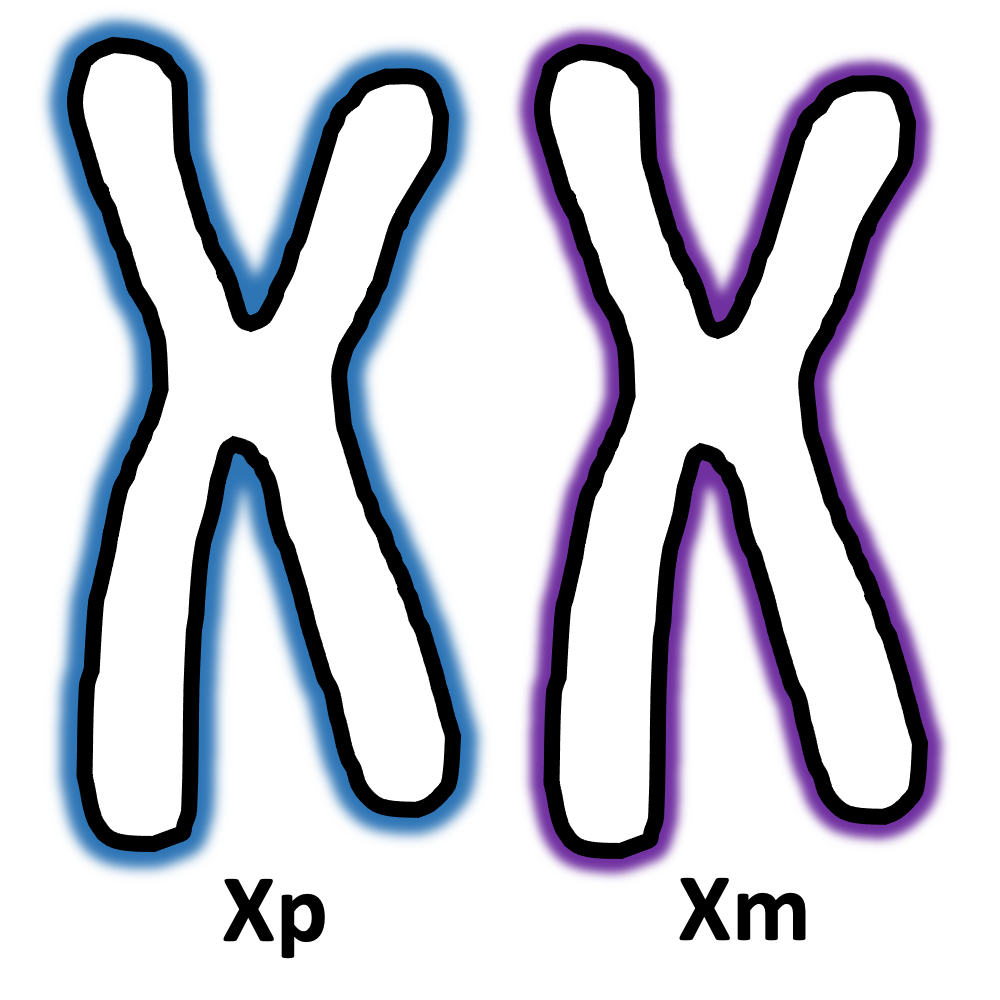
\includegraphics[width=0.2\textwidth,height=\textheight]{images/XCI-images/Slide2.png}\\
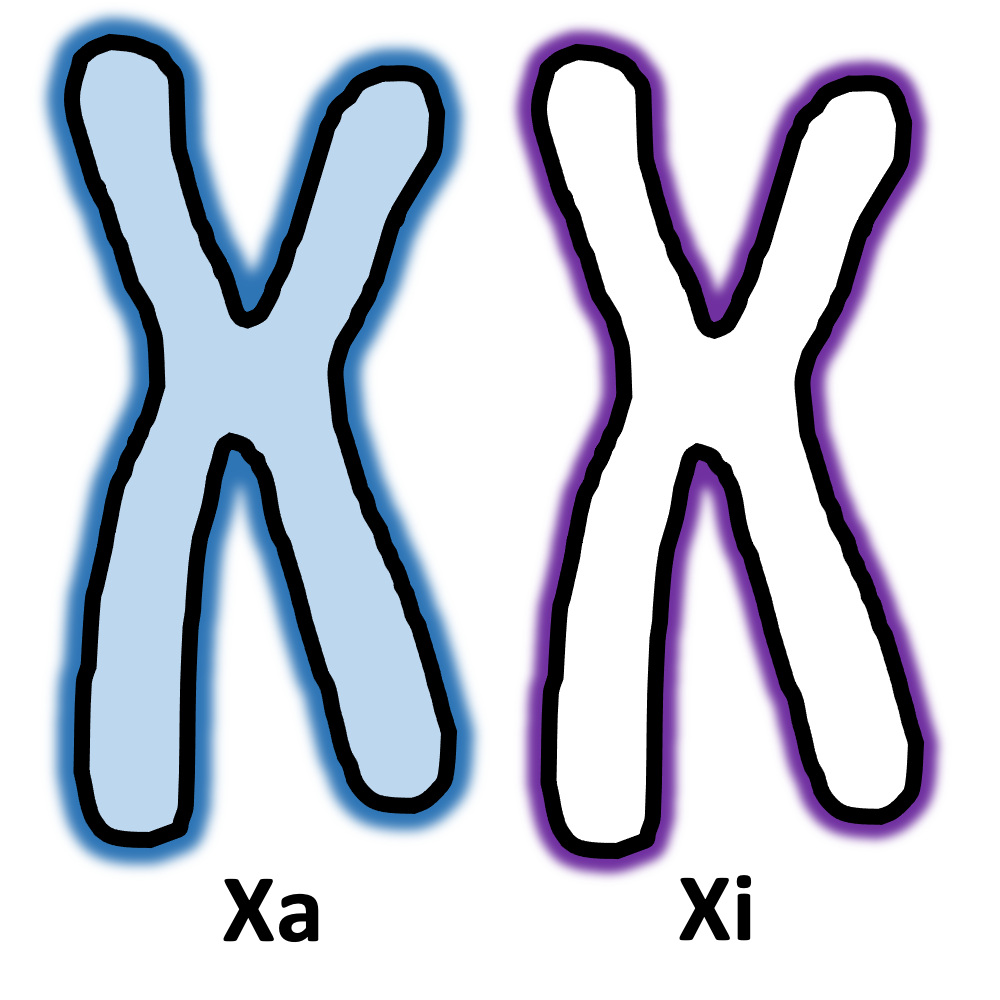
\includegraphics[width=0.12\textwidth,height=\textheight]{images/XCI-images/Slide3.png}
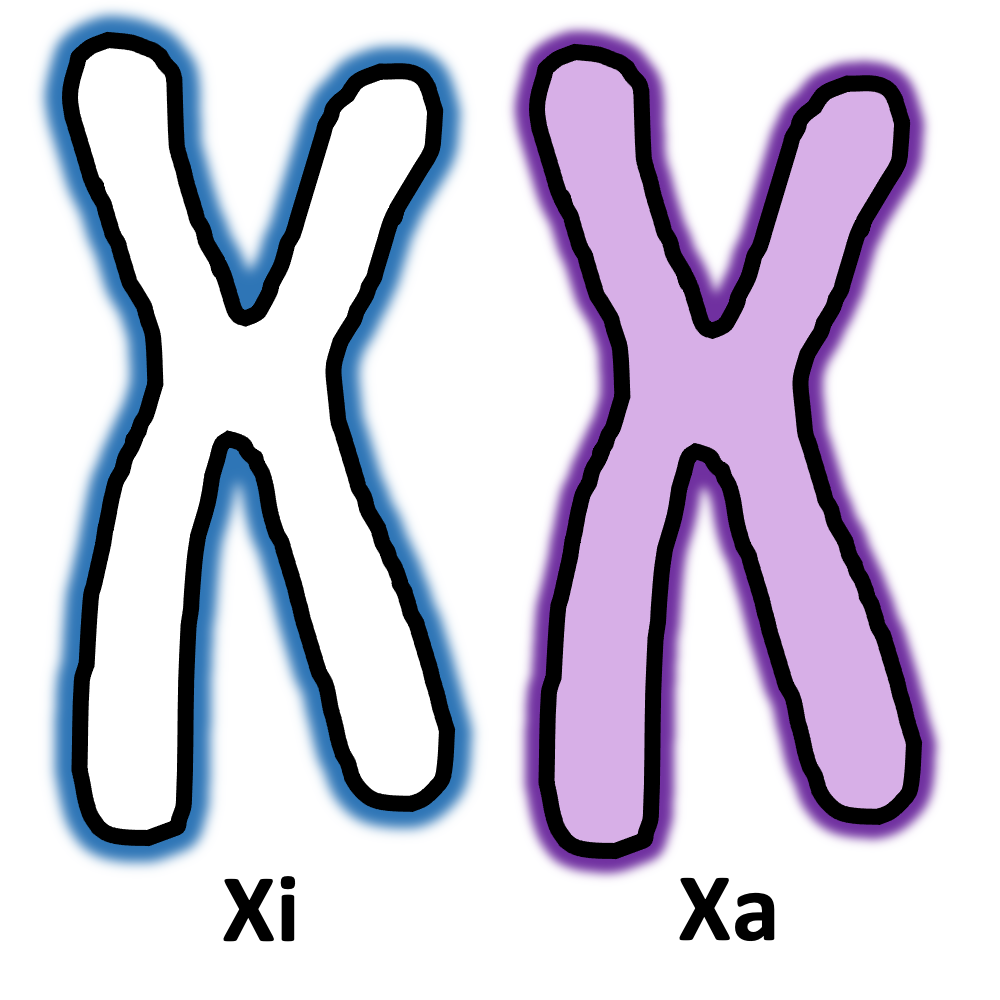
\includegraphics[width=0.12\textwidth,height=\textheight]{images/XCI-images/Slide4.png}\\

\textbf{\emph{Figure 1: The paternally inherited (Xp) chromosome in and
the maternally inherited chromosome (Xm).}}~ \emph{The active chromosome
Xa is represented with color filled in, while the
inactive}~\emph{chromosome Xi is represented with no color fill.}\\

\textbf{Escape}: The status of genes which are expressed on Xi. These
genes ``escape'' inactivation.

\textbf{Inactive}: The status of genes which are suppressed on Xi.

\textbf{Variable}: The status of genes which are expressed on Xi in some
tissues/individuals,\\
but not in all tissues/individuals. {[}2{]}

\textbf{Mosaicism}: Xa and Xi are typically randomly assigned to either
Xp or Xm in each\\
cell. \emph{Mosaicism} refers to the heterogeneity of Xa/Xi assignment
among a set of cells.

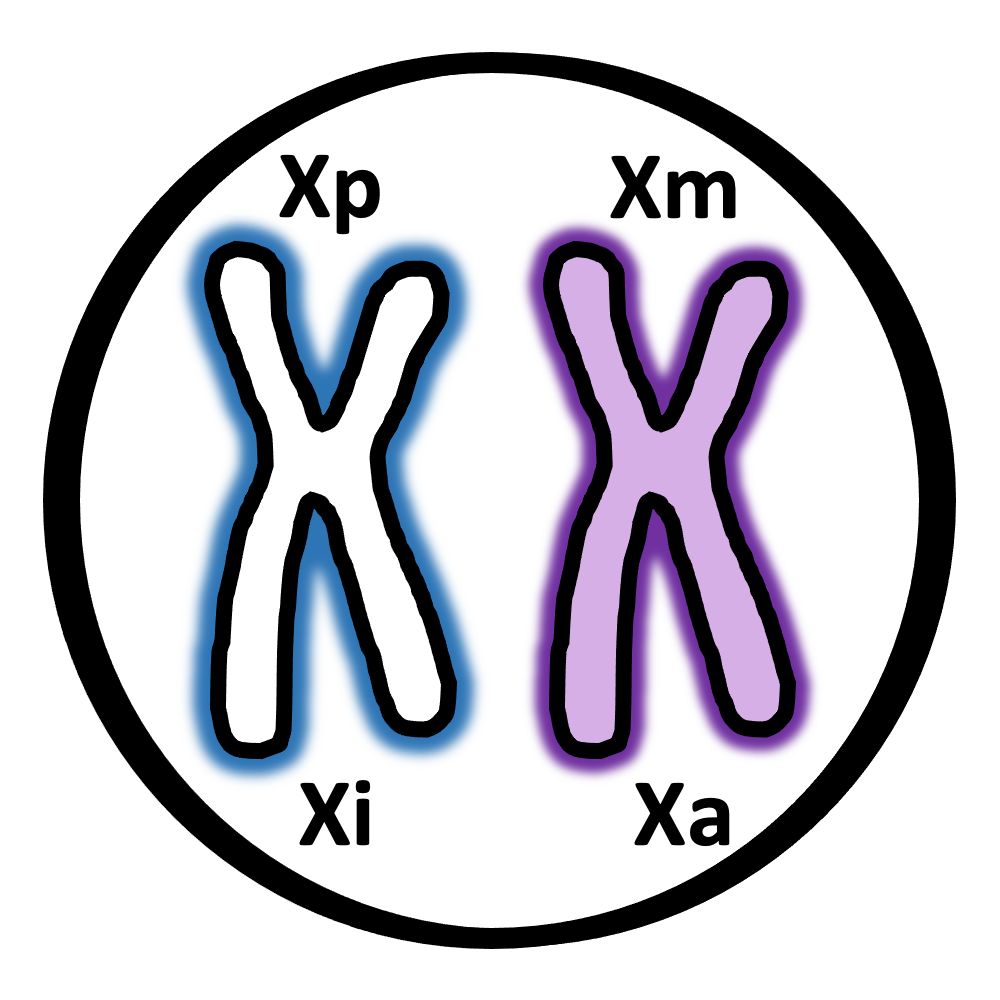
\includegraphics[width=0.1\textwidth,height=\textheight]{images/XCI-images/Slide5.png}
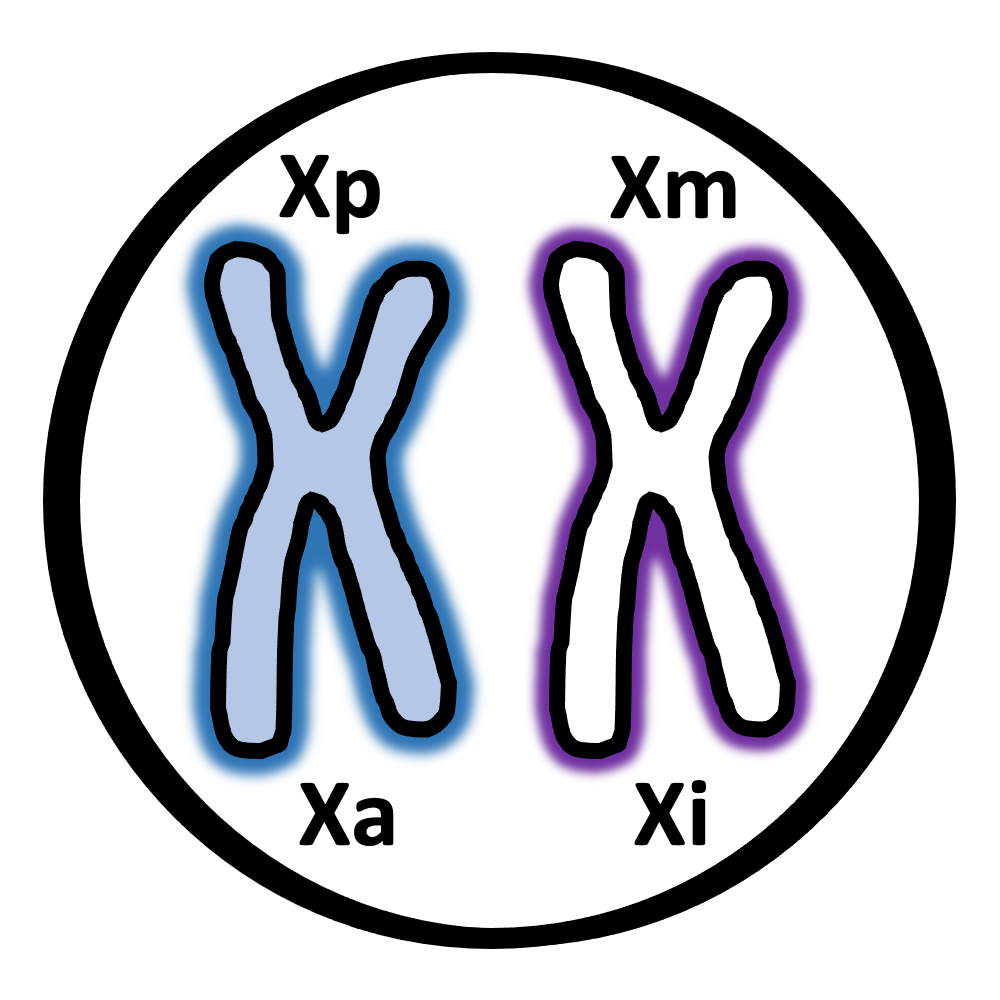
\includegraphics[width=0.1\textwidth,height=\textheight]{images/XCI-images/Slide6.png}
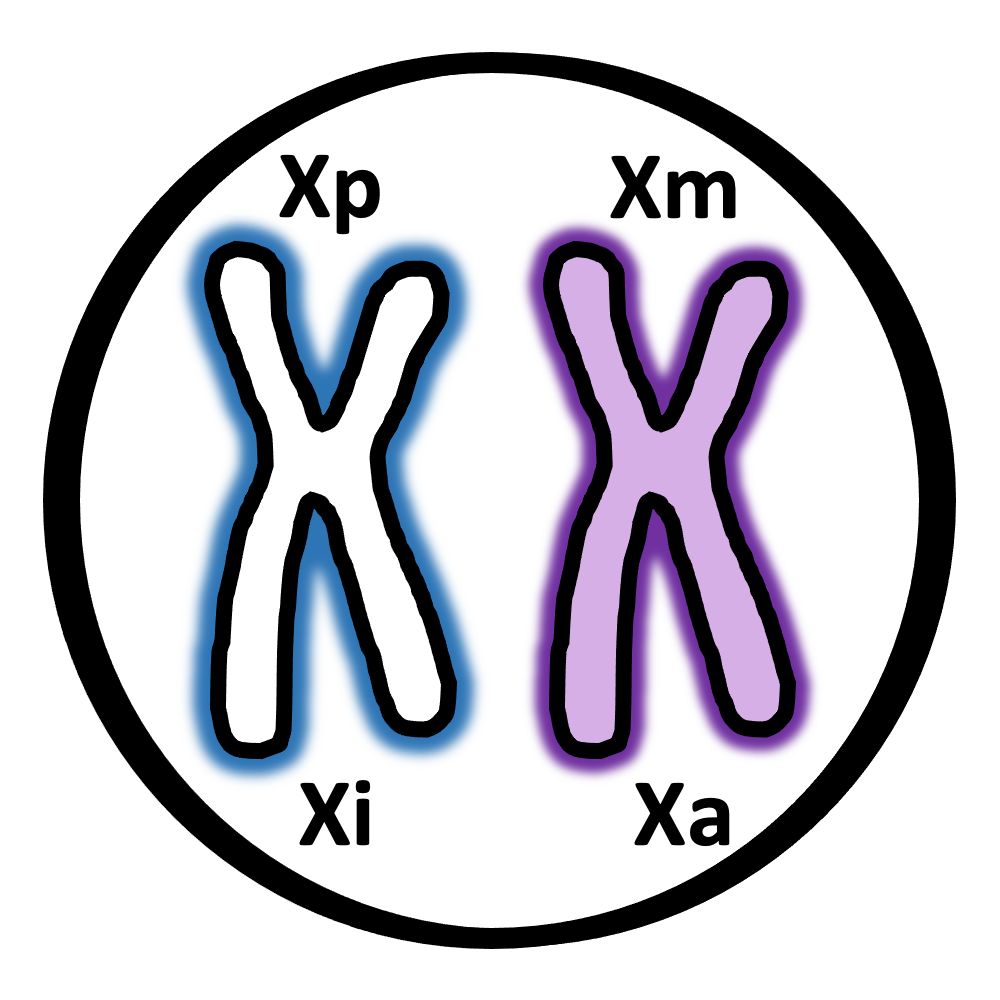
\includegraphics[width=0.1\textwidth,height=\textheight]{images/XCI-images/Slide5.png}
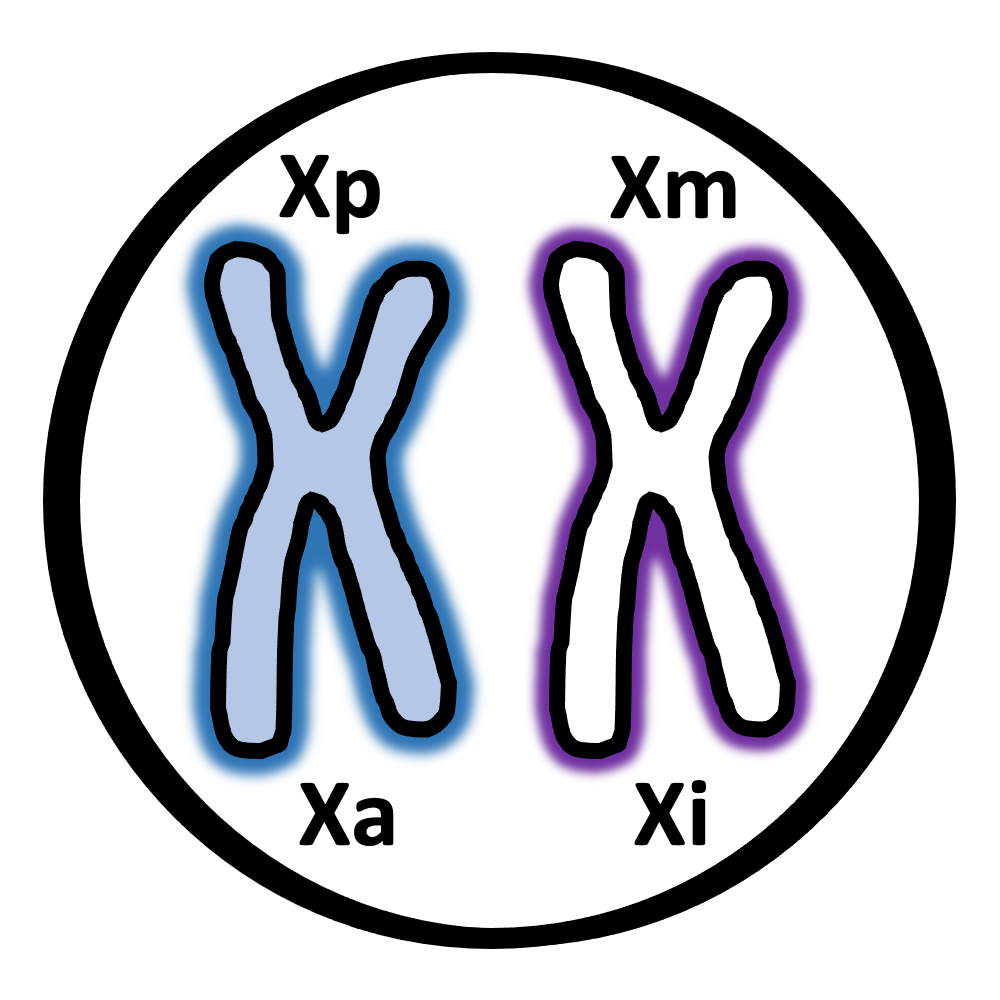
\includegraphics[width=0.1\textwidth,height=\textheight]{images/XCI-images/Slide6.png}\\
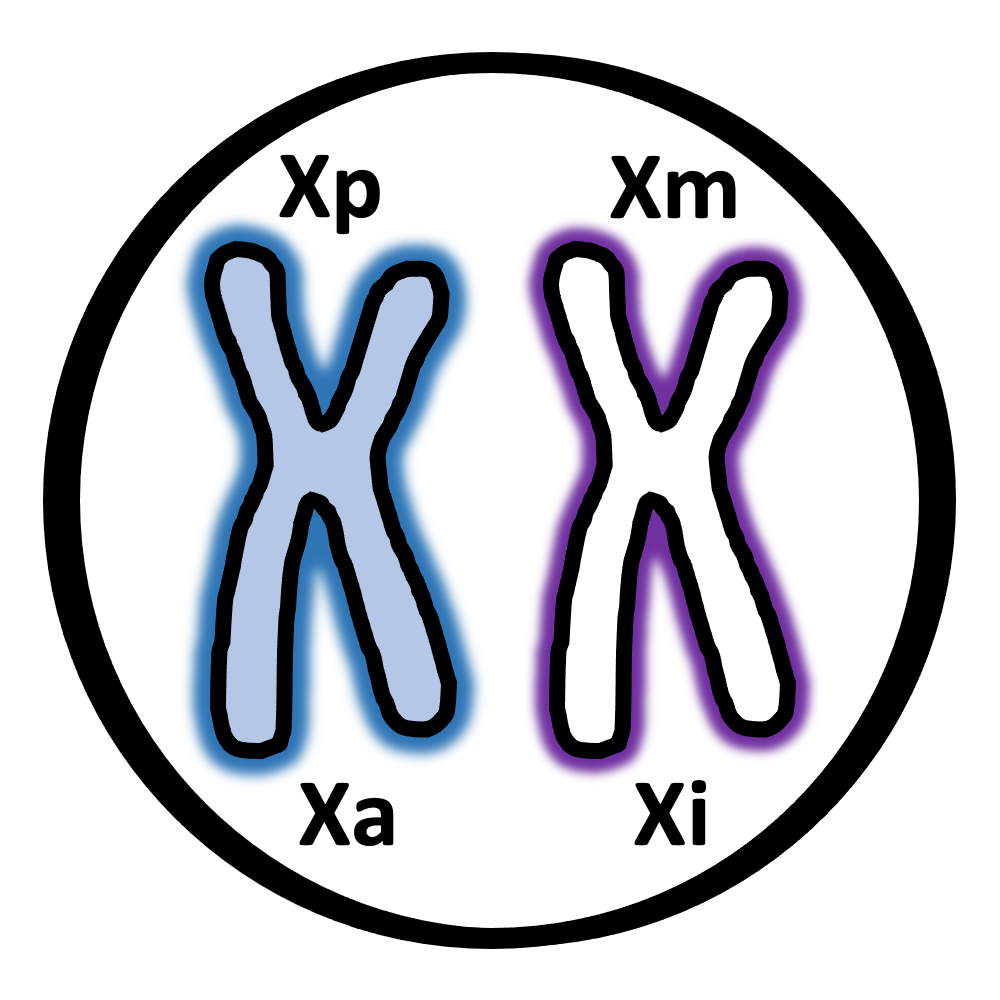
\includegraphics[width=0.1\textwidth,height=\textheight]{images/XCI-images/Slide6.png}
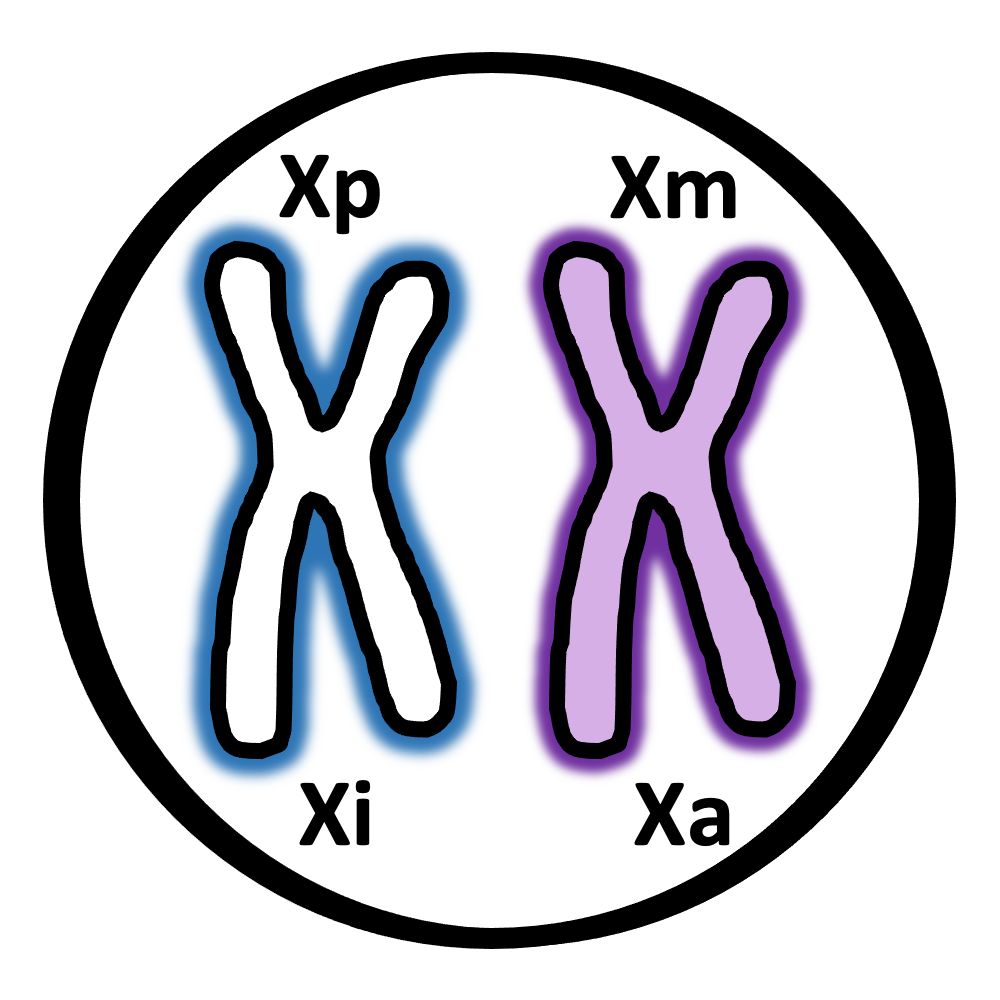
\includegraphics[width=0.1\textwidth,height=\textheight]{images/XCI-images/Slide5.png}
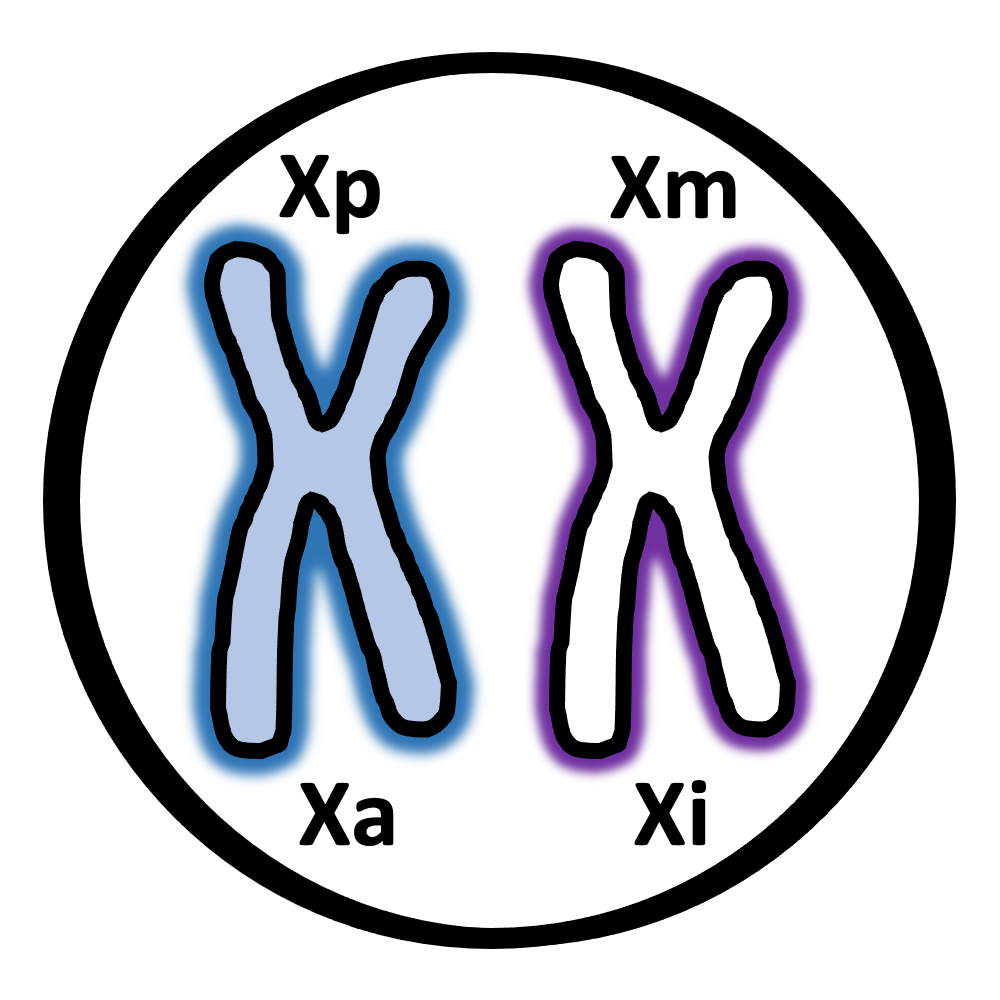
\includegraphics[width=0.1\textwidth,height=\textheight]{images/XCI-images/Slide6.png}
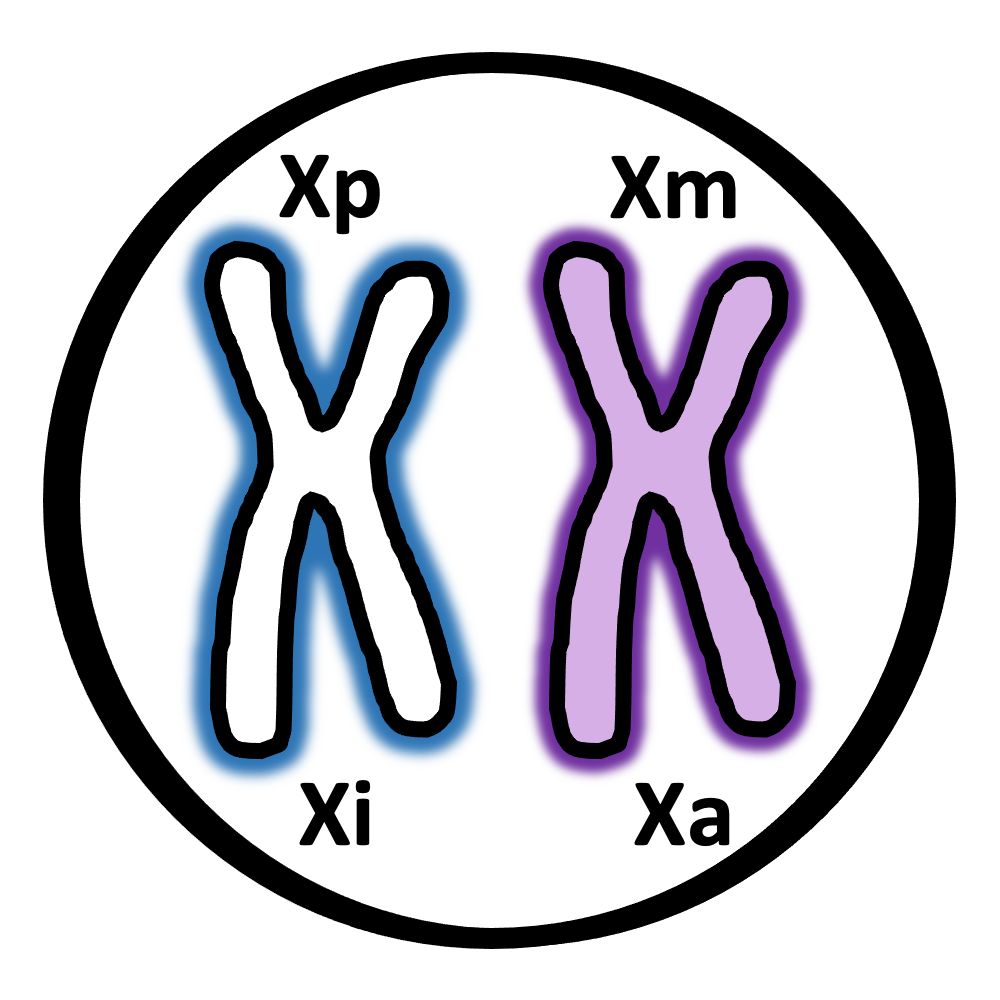
\includegraphics[width=0.1\textwidth,height=\textheight]{images/XCI-images/Slide5.png}\\
\textbf{\emph{Figure 2: Mosaicism.}} \emph{A sample of six cells with
differences in Xa/Xi assignments.}\\

\textbf{Skew}: A ratio which represents the mosaicism of Xa/Xi
assignment in a\\
set of cells.

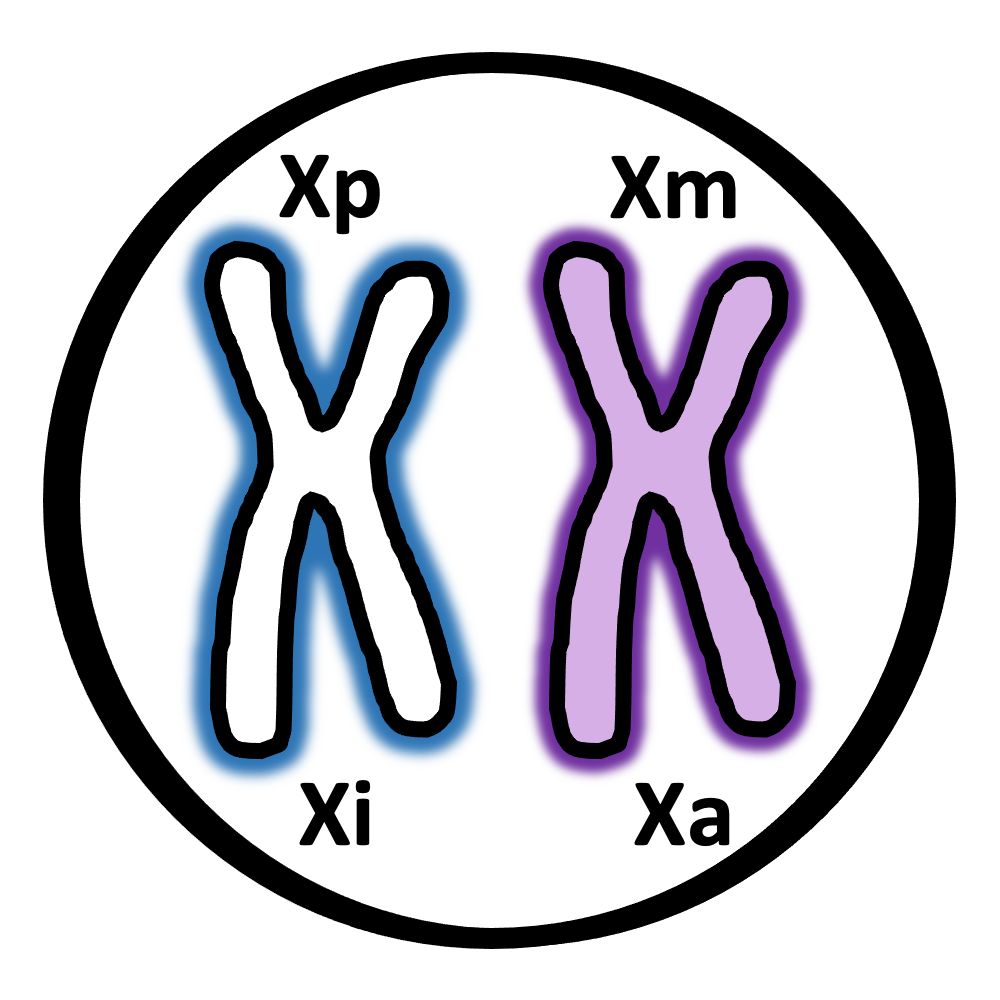
\includegraphics[width=0.12\textwidth,height=\textheight]{images/XCI-images/Slide5.png}
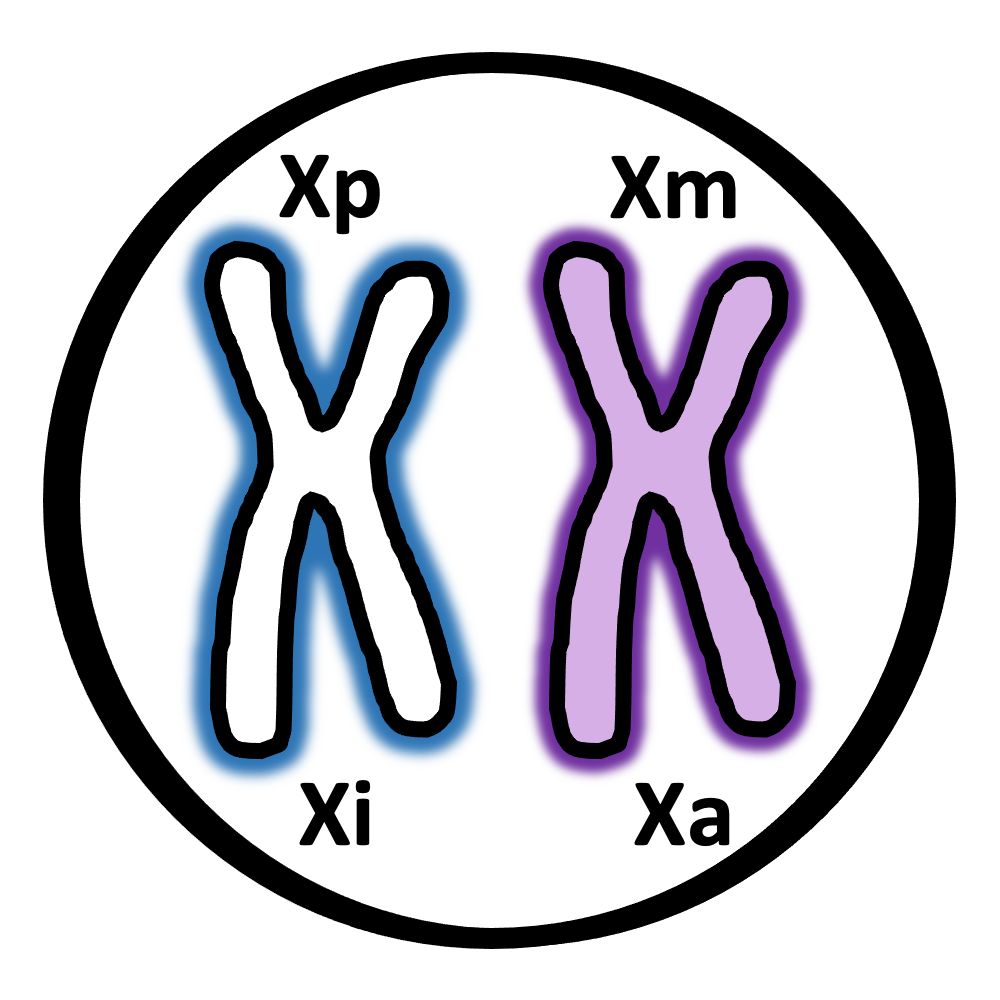
\includegraphics[width=0.12\textwidth,height=\textheight]{images/XCI-images/Slide5.png}
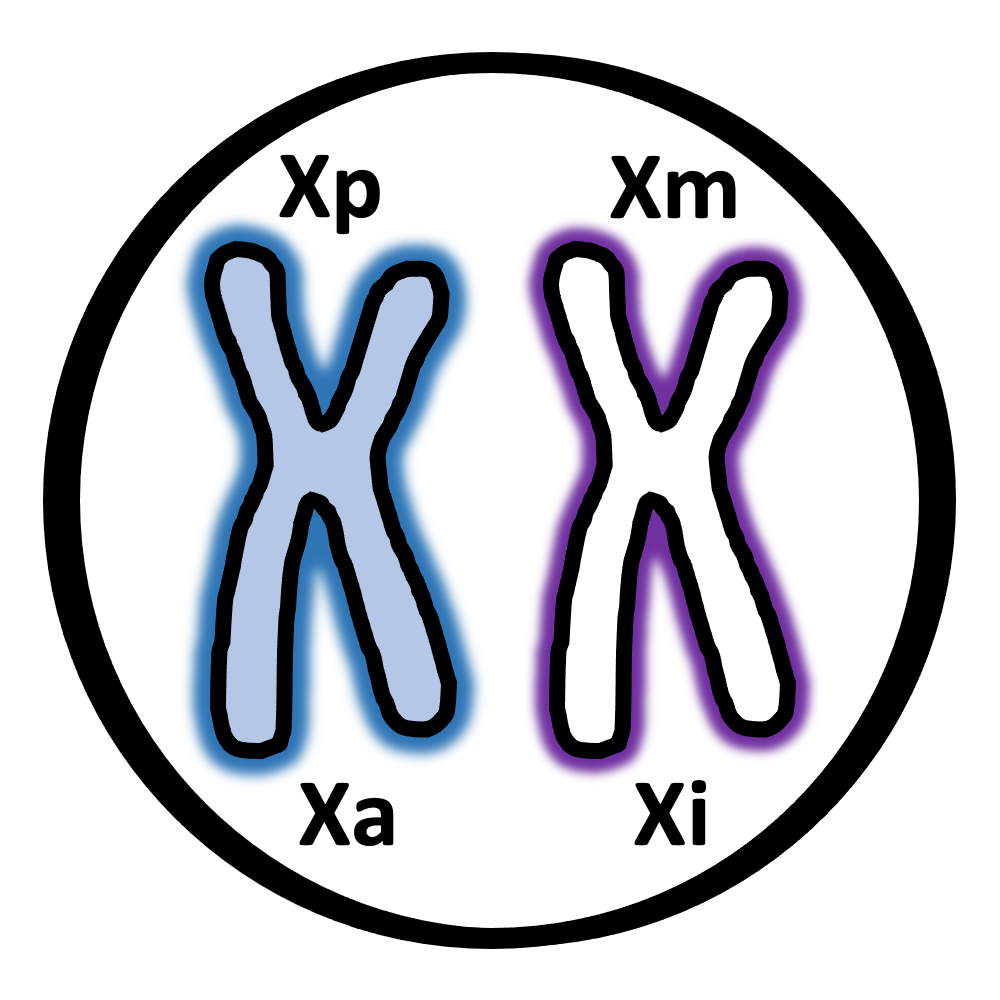
\includegraphics[width=0.12\textwidth,height=\textheight]{images/XCI-images/Slide6.png}
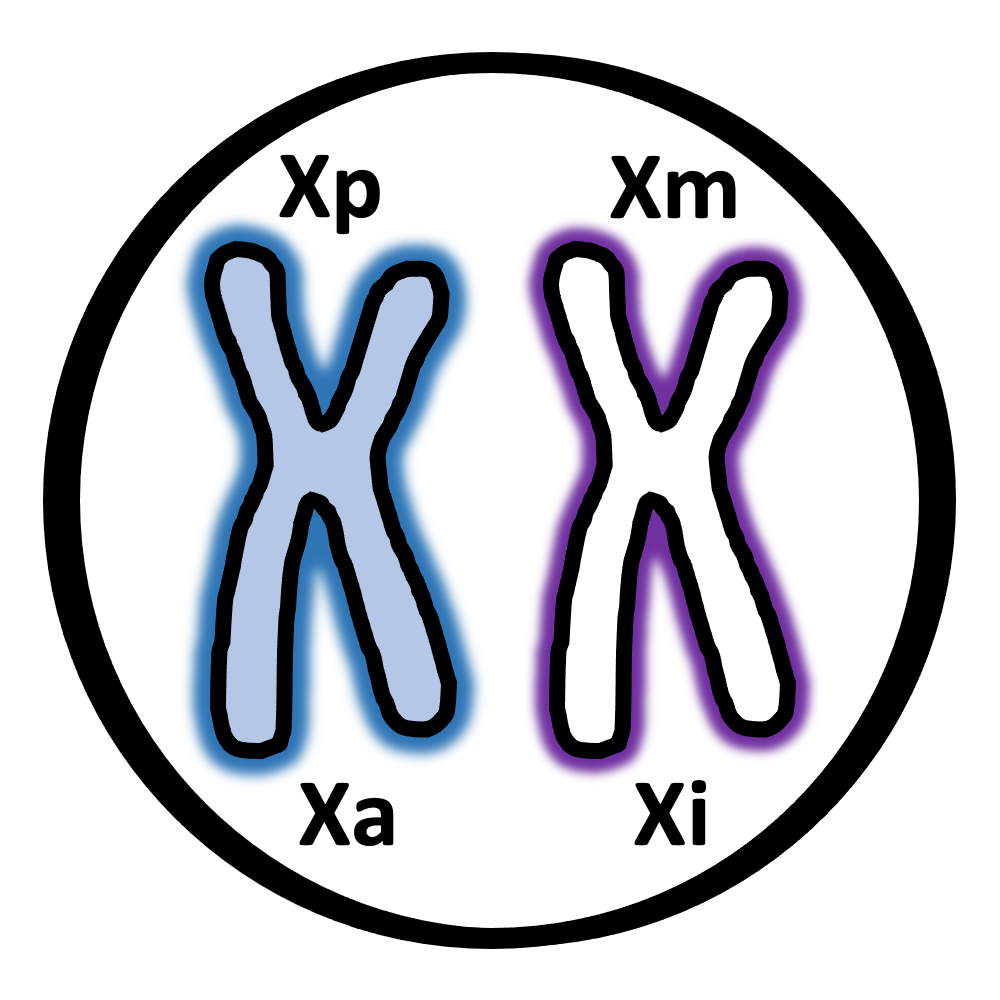
\includegraphics[width=0.12\textwidth,height=\textheight]{images/XCI-images/Slide6.png}\\
\textbf{\emph{Figure 3a: Skew Ratio 1.}} \emph{Two samples have Xi
assignment on Xm, while two samples}\\
\emph{have Xi assignment on Xp. The resulting skew ratio is 50:50.}

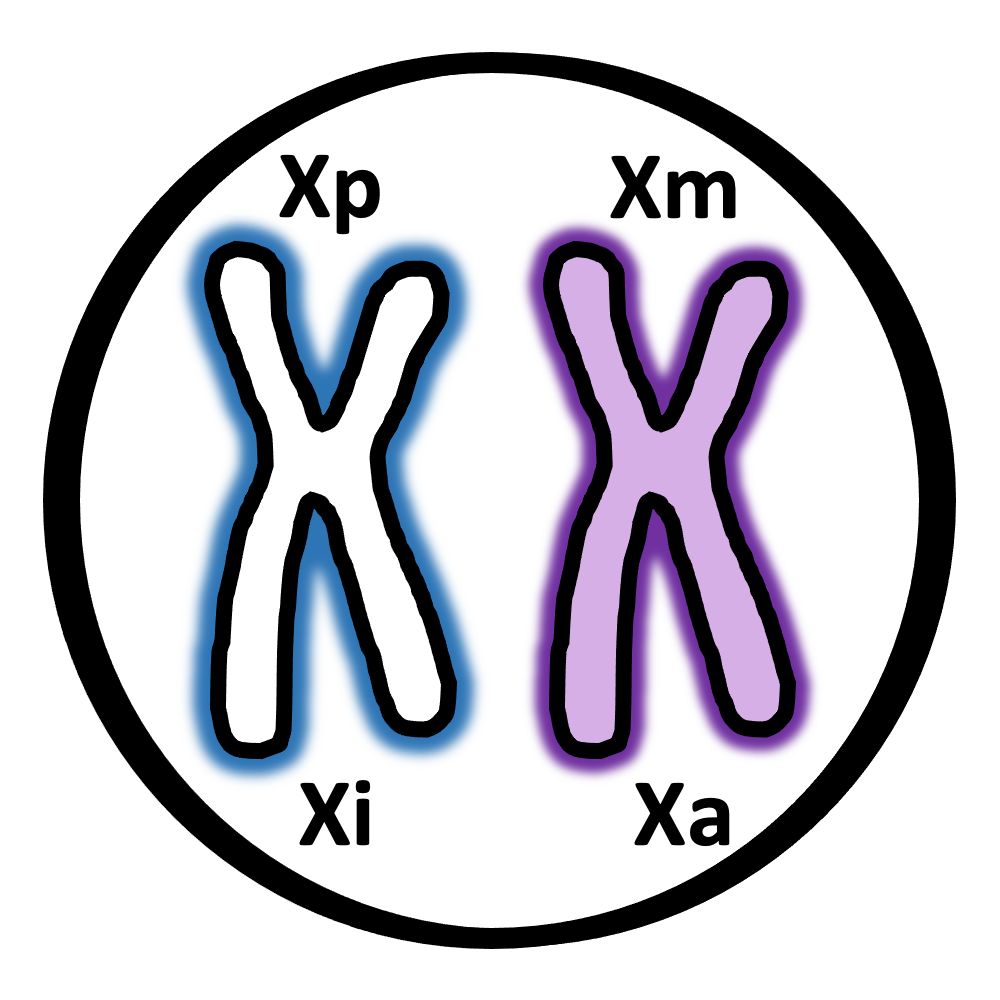
\includegraphics[width=0.12\textwidth,height=\textheight]{images/XCI-images/Slide5.png}
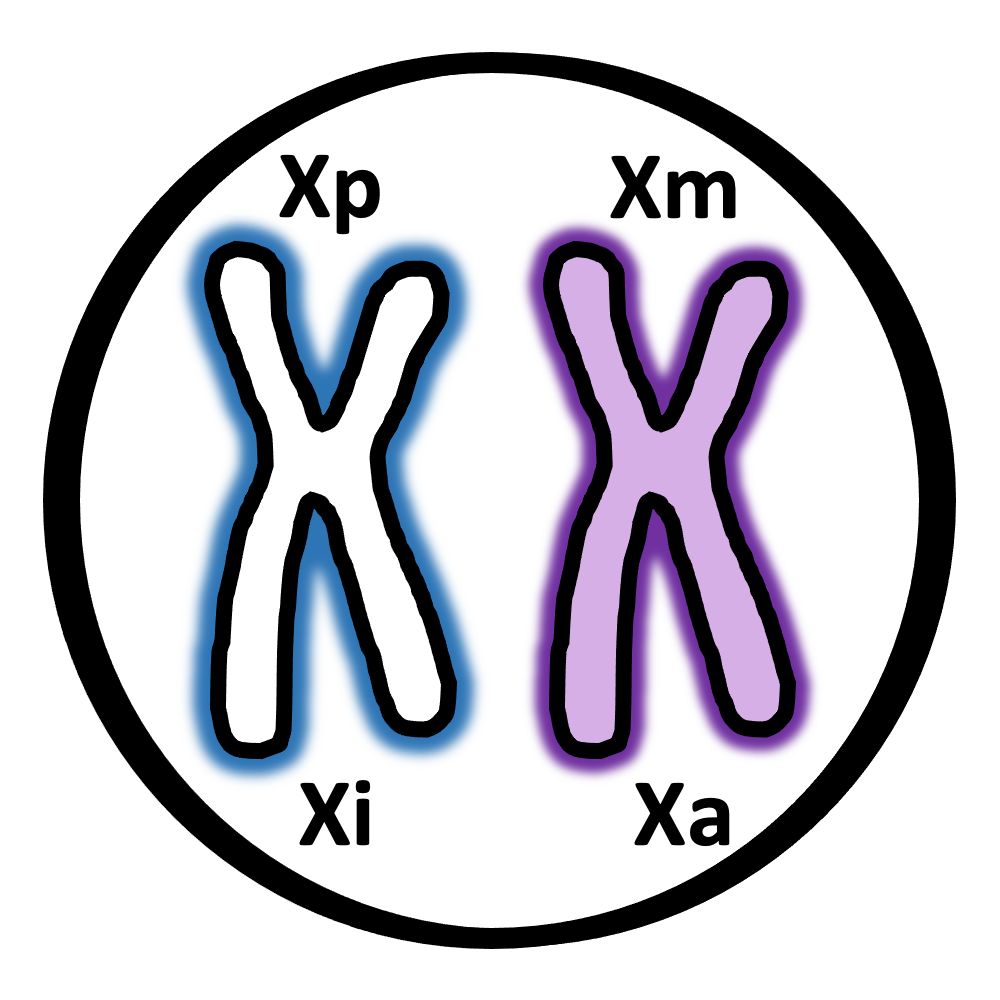
\includegraphics[width=0.12\textwidth,height=\textheight]{images/XCI-images/Slide5.png}
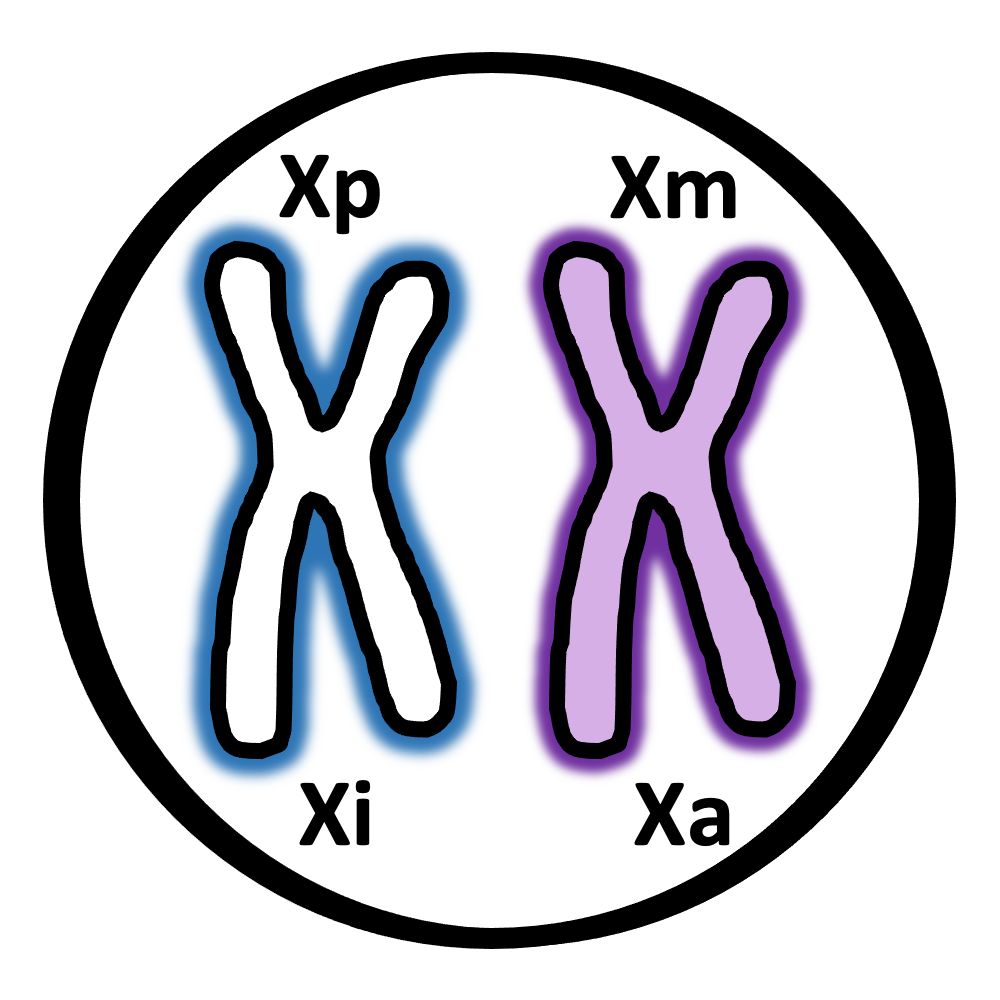
\includegraphics[width=0.12\textwidth,height=\textheight]{images/XCI-images/Slide5.png}
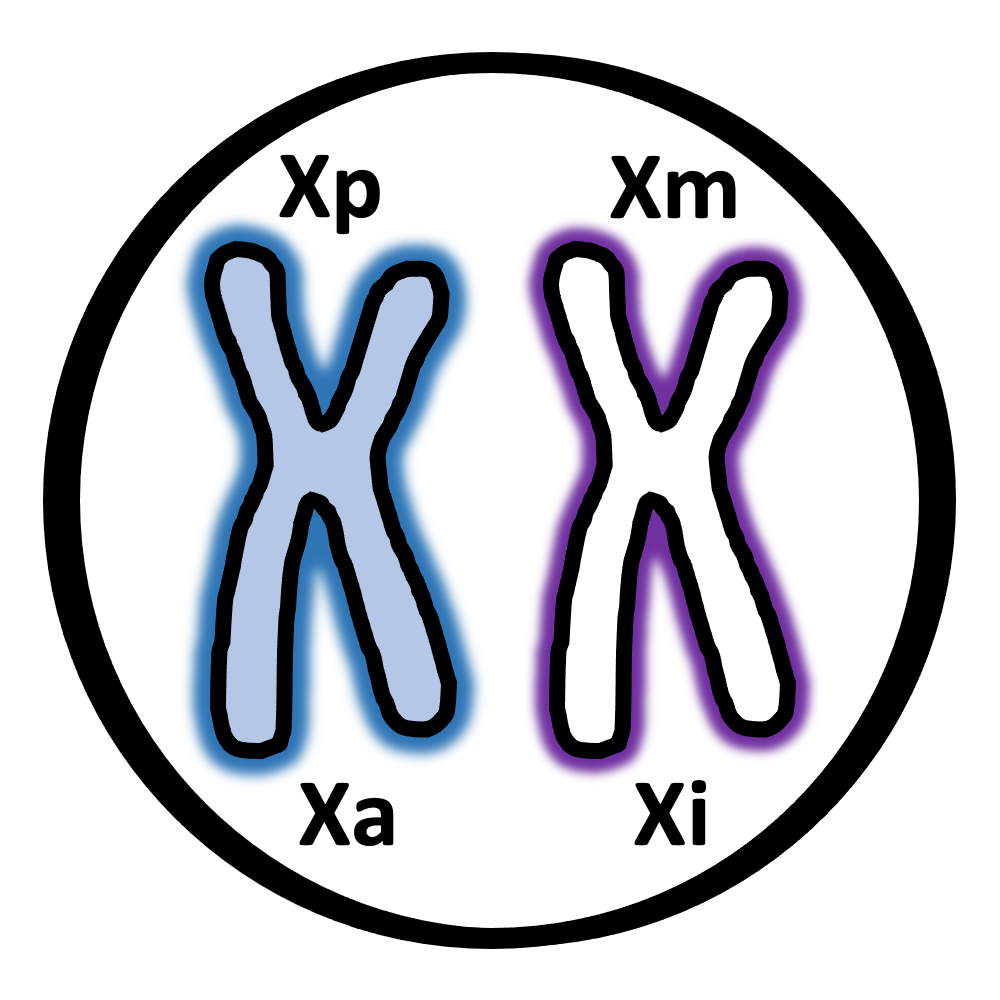
\includegraphics[width=0.12\textwidth,height=\textheight]{images/XCI-images/Slide6.png}\\
\textbf{\emph{Figure 3b: Skew Ratio 2.}} \emph{Three samples have Xi
assignment on Xm, while one sample}\\
\emph{has Xi assignment on Xp. The resulting skew ratio is 25:75.}

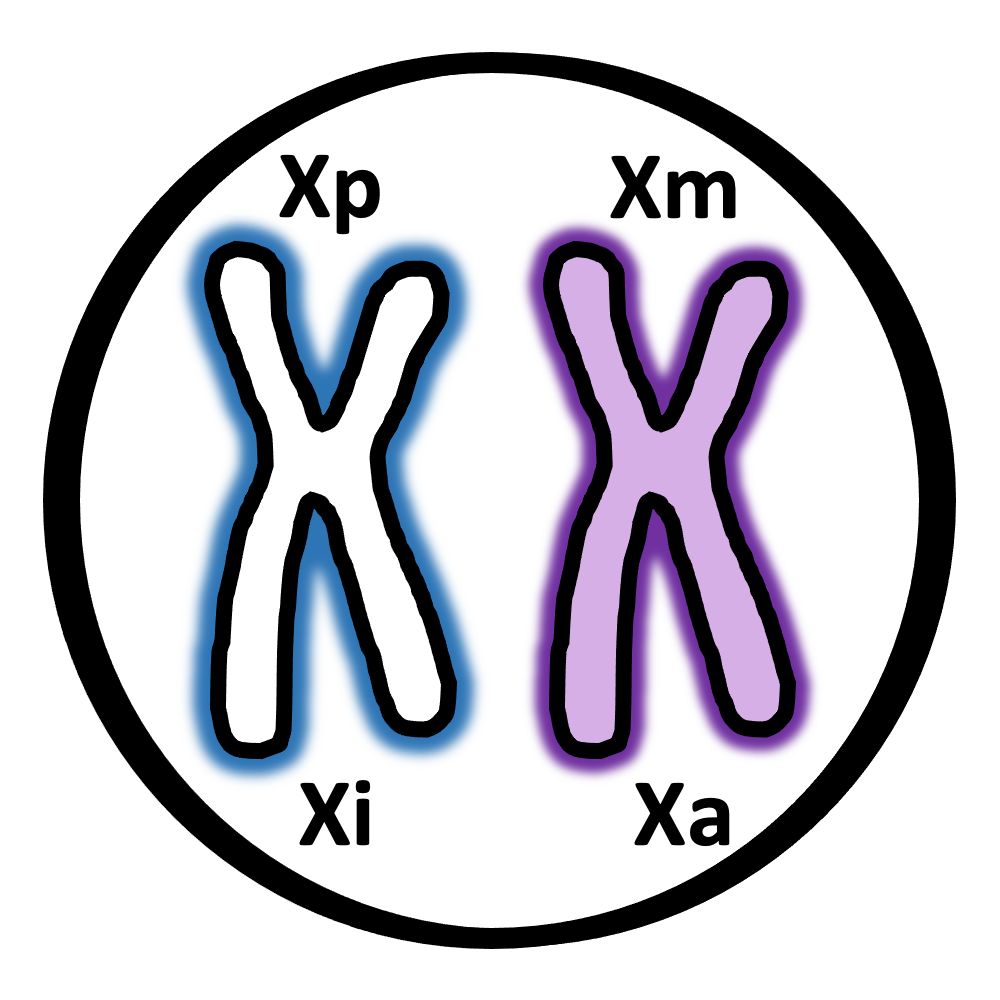
\includegraphics[width=0.12\textwidth,height=\textheight]{images/XCI-images/Slide5.png}
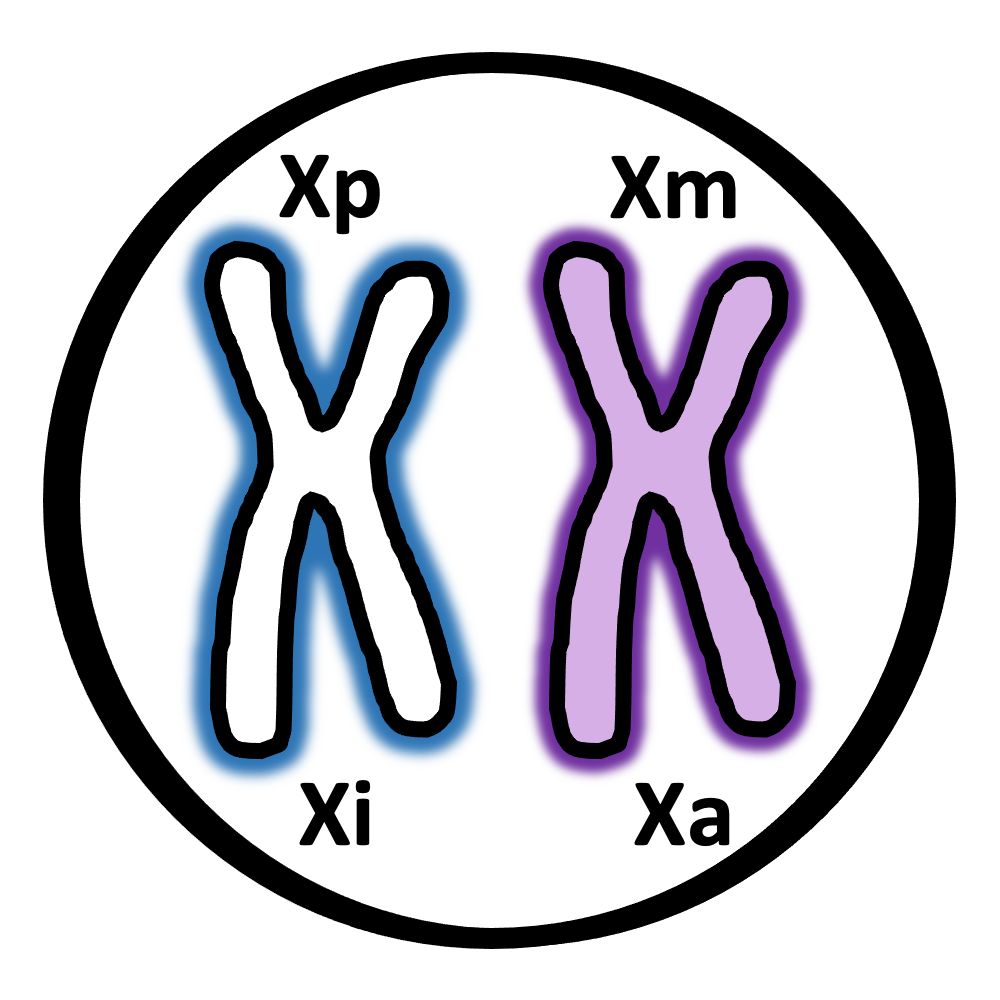
\includegraphics[width=0.12\textwidth,height=\textheight]{images/XCI-images/Slide5.png}
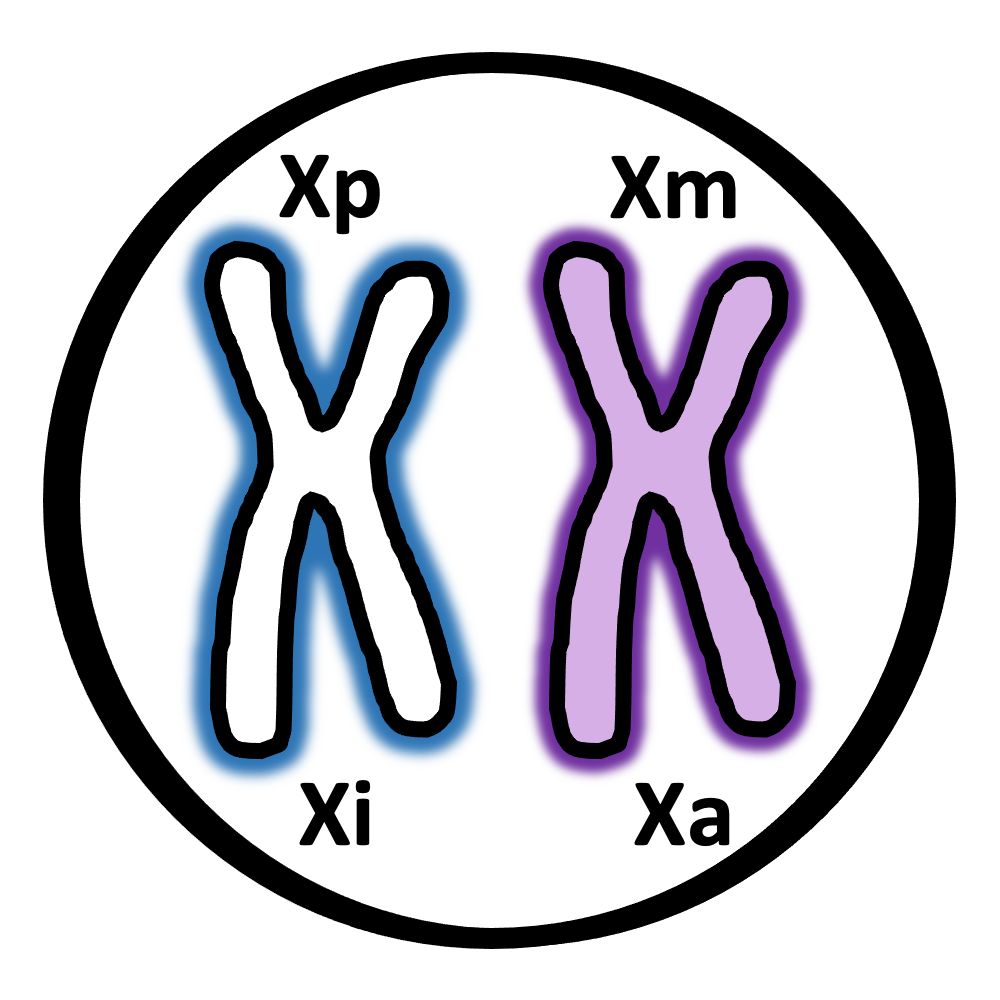
\includegraphics[width=0.12\textwidth,height=\textheight]{images/XCI-images/Slide5.png}
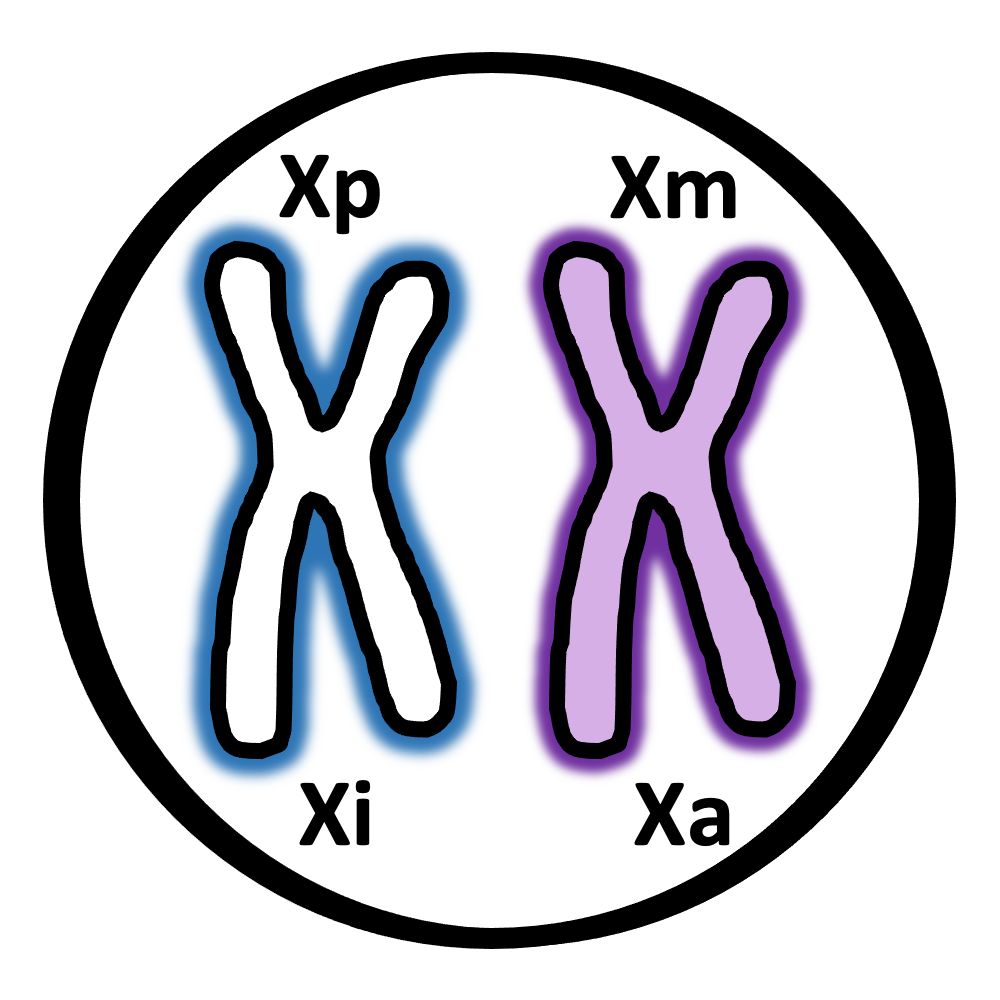
\includegraphics[width=0.12\textwidth,height=\textheight]{images/XCI-images/Slide5.png}\\
\textbf{\emph{Figure 3c: Skew Ratio 2.}} \emph{All four samples have Xi
assignment on Xm.}\\
\emph{The resulting skew ratio is 0:100. This is a rare occurrence in
nature, and is often}~\emph{referred to has non-random assignment or a
fully skewed individual. {[}3{]}}

\textbf{Tau (\(\tau\))}: The ratio of a gene's expression on Xi over its
total expression across\\
both Xa and Xi. In allele specific expression (ASE) based methods for
escape inference,\\
\(\tau\) is compared to the skew ratio. Significant deviation of
\(\tau\) from the skew~ ratio reflects biallelic expression and
classifies a gene as escape.

\(N=expression\ level\)

\(j=gene\)

\(i=inactive\ x\ chromosome\)

\(a=active\ x\ chromosome\)

\(\tau = \frac{N_{ij}}{N_{aj} + N_{ij}}\)

\emph{A note about skew: For ASE based methods, data sets with a higher
skew ratio (such as 25:75)}\\
\emph{are strengthened for estimating escape expression due to the lower
Xi expression levels}~ \emph{required to infer significance.}

\textbf{Tau+ (\(\tau\)+)}: The \(\tau\) values from the subset of XCI
calls which were inferred from\\
samples which were sufficiently skewed (\textgreater25:75). This subset
is a more robust estimate of\\
ASE and is strengthened for escape calling.

{[}1{]} LYON MF. Gene action in the X-chromosome of the mouse (Mus
musculus L.). \emph{Nature.} 1961;190:372-373.
\href{https://www.nature.com/articles/190372a0}{doi:10.1038/190372a0}\\
{[}2{]} Carrel L, Brown CJ. When the Lyon(ized chromosome) roars:
ongoing expression from an inactive X chromosome. \emph{Philos Trans R
Soc Lond B Biol Sci.} 2017;372(1733):20160355.
\href{https://royalsocietypublishing.org/doi/10.1098/rstb.2016.0355}{doi:10.1098/rstb.2016.0355}\\
{[}3{]} Tukiainen T, Villani AC, Yen A, et al.~Landscape of X chromosome
inactivation across human tissues {[}published correction appears in
\emph{Nature.} 2018 Mar 7;555(7695):274{]}. \emph{Nature.}
2017;550(7675):244-248.
\href{https://doi.org/10.1038/nature24265}{doi:10.1038/nature24265}

\end{document}
